% Ubah kalimat sesuai dengan judul dari bab ini
\chapter{DESAIN DAN IMPLEMENTASI}

% Ubah konten-konten berikut sesuai dengan yang ingin diisi pada bab ini

\section{Deskripsi Sistem}

Sistem kami bernama JagaBersama, suatu sistem yang dapat digunakan untuk mendeteksi kekerasan baik itu merupakan kekerasan dalam rumah tangga maupun \textit{bullying} atau perundungan yang biasa terjadi di sekolah - sekolah maupun di tempat umum. Dengan memanfaatkan salah satu cabang dalam pembelejaran mesin yaitu \textit{Deep Learning} ditambah dengan pengolahan citra modern, kita dapat melakukan pendeteksian secara otomatis dengan cepat dan murah. Diharapkan dengan adanya sistem kami maka dapat mengurangi jumlah kasus kekerasan di Indonesia dan dapat memberikan suatu ide pendekatan yang baru dalam menanggulangi kekerasan di Indonesia.

Terdapat 2 target pengguna dalam sistem kami, yang pertama adalah Pengguna Umum yang akan memasang sistem kami (kamera + \textit{raspberry pi}) yang akan dapat secara otomatis mendeteksi kekerasan. Kemudian target pengguna yang pertama adalah Agen, agen disini yang dimaksud adalah agen yang dapat berasal dari Komnas Perempuan yang bertugas untuk menyelesaikan apabila terjadi suatu kasus kekerasan maupun bisa juga agen lain seperti polisi atau guru apabila kekerasan terjadi di sekolah.

Namun, sebagai catatan, tanggung jawab saya kebanyakan merupakan pada bagian membuat aplikasi Android yang digunakan sebagai antar-muka antar agen dengan sistem basis data secara keseluruhan.

\section{Implementasi Alat}

Terdapat 3 bagian terpisah dari sistem kami yang semuanya bekerja secara bersamaan sehingga menciptakan suatu sistem yang dapat berjalan dengan lancar dan \textit{reliable}. Bagian pertama adalah bagian \textit{Internet of Things} (IoT), selanjutnya adalah \textit{server} sebagai bagian paling penting dalam keseluruhan sistem dan terakhir adalah aplikasi Android sebagai antar-muka dengan agen. Gambar \ref{fig:framework} adalah gambaran secara luas bagaimana sistem kami bekeja secara keseluruhan.


\begin{figure} [!ht]
  \centering
  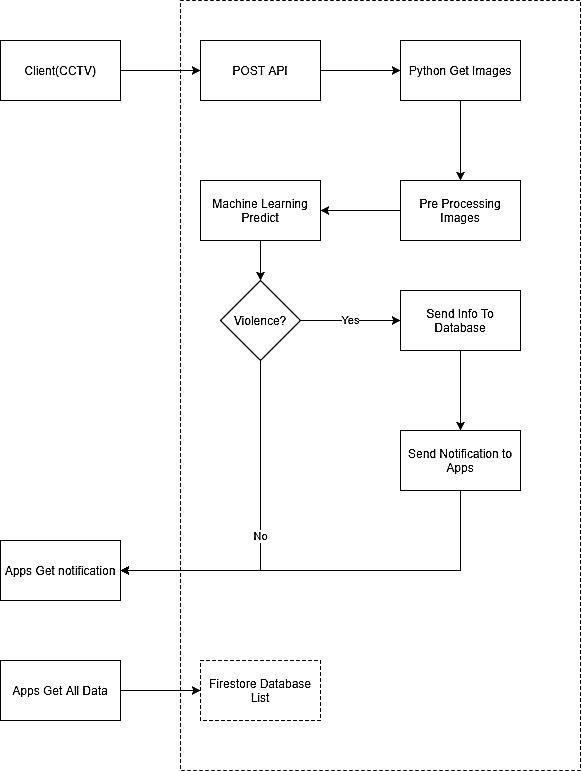
\includegraphics[width=0.8\textwidth]{gambar/framework.jpg}
  % Keterangan gambar yang diinputkan
  \caption{Diagram \textit{Framework} Keseluruhan Proyek}
  % Label referensi dari gambar yang diinputkan
  \label{fig:framework}
\end{figure}

\subsection{Implementasi IoT}

Dalam proyek ini kami berencana untuk menggunakan 2 tipe alat, yang pertama adalah menggunakan CCTV ditambah dengan Raspberry Pi, yang kedua adalah menggunakan CCTV ditambah dengan Jetson Nano yang notabene lebih mahal dibanding alat pertama. Alasan kami memiliki 2 alat adalah kami ingin memberikan pengguna suatu pilihan. Apabila menggunakan Raspberry Pi maka nantinya Raspberry Pi akan mengirimkan foto ke \textit{server} kami setiap beberapa menit sekali sehingga dari sisi \textit{privacy}, hal ini cukup mengkhawatirkan karena walaupun \textit{server} kami sama sekali tidak menyimpan foto dalam jangka waktu yang lama kecuali apbaila dalam foto tersebut terdeteksi adanya kekerasan, namun seseorang dapat melancarkan \textit{Man in The Middle Attack} (MITM), yang berarti seseorang 'menguping' seluruh permintaan koneksi dari \textit{server} ke Raspberry Pi. Alat kedua memiliki tingkat \textit{privacy} yang lebih baik, karena Jetson Nano memiliki kemampuan untuk melakukan deteksi secara \textit{on-device} sehingga hanya mengirimkan data atau foto apabila terdapat kekerasan terdeteksi.